\selectlanguage{italian}%

\section{Simulazione}

In Figura \ref{fig:scan_chain_sim} � osservabile il funzionamento
del sistema appena descritto, utilizzando il testbench presente al
seguente link: \href{run:progetti/Boundary_Scan_Chain/boundary_scan_chain_testbench.vhd}{Boundary\_Scan\_Chain\_Testbench}.
\\
Come si nota � stata abilitata la modalit� shift register ponendo
ad 1 sia \textit{en}, che \textit{scan\_en}, in modo da shiftare il
valore 1 posto in ingresso a \textit{scan\_in}, che � visibile all'uscita
scan\_out esattamente dopo quattro colpi di clock, come c'era d'aspettarsi
dato che il numero di flip flop utilizzati � proprio quattro. Dopodich�
si � scelto di abilitare la modalit� registro e quindi a 55 ns sono
stati abbassati sia \textit{en} che \textit{scan\_en} e difatti all'uscita
\textit{dout} dei flip flop si osserva il valore 1010 posto in ingresso
precedentemente a \textit{din}.

\begin{figure}[H]
	\centering
	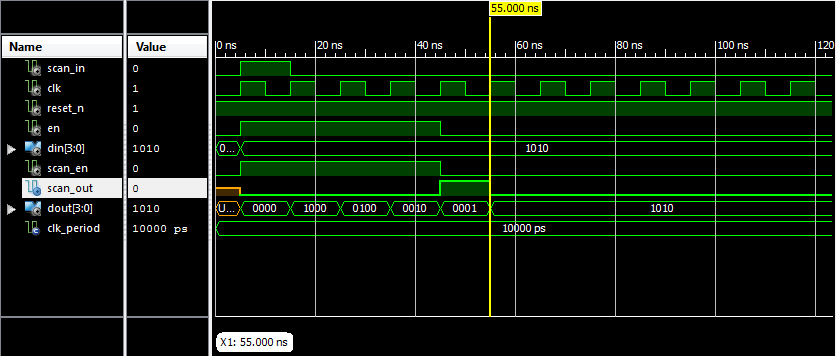
\includegraphics[scale=0.8]{esercizio06/images/scan_chain_simulazione.png}
	\caption{Simulazione della Boundary Scan Chain Behavioral}
	\label{fig:scan_chain_sim}
\end{figure}\selectlanguage{italian}%

